\pdfminorversion=7
\documentclass[preprint,11pt]{elsarticle}
\usepackage[margin=1in]{geometry}
\usepackage[T1]{fontenc}
\usepackage{lmodern}
\input{glyphtounicode}
\pdfgentounicode=1
\usepackage{amsmath,amssymb,bm,booktabs,graphicx,siunitx,etoolbox}
\usepackage[expansion=false]{microtype}
\usepackage{array,longtable,setspace,xurl,hyperref,caption,placeins,lineno,float}
\usepackage{tikz}
\usetikzlibrary{arrows.meta,positioning,calc}
\newfloat{algorithm}{!htbp}{loa}
\floatname{algorithm}{Algorithm}
\hypersetup{
  hidelinks,
  pdftitle={Correcting frozen-state curvature in inverse physics-informed neural networks via regularized state elimination},
  pdfauthor={Ziwei Ren, Shijin Zhang, Ming Chen, Chuangrui Zheng}
}
\robustify\bfseries
\sisetup{group-digits=false,detect-weight=true,detect-family=true}
\newcommand{\doi}[1]{doi:\,\mbox{\href{https://doi.org/#1}{\nolinkurl{#1}}}}
\newcommand{\RR}{\mathbb R}
\captionsetup{font=small,labelfont=bf}
\setstretch{1.08}
\raggedbottom
\setlength{\emergencystretch}{2em}
\setlength{\parskip}{2pt}
\setcounter{topnumber}{3}\setcounter{totalnumber}{5}
\renewcommand{\topfraction}{.92}\renewcommand{\textfraction}{.06}
\renewcommand{\floatpagefraction}{.78}
\newcommand{\rbar}{\bar{\bm r}}
\newcommand{\Jt}{J_\theta}\newcommand{\Jl}{J_\lambda}
\newcommand{\Fraw}{F_{\mathrm{raw}}}
\newcommand{\Fse}{F_{\mathrm{se}}^{\mathrm{GN}}}
\newcommand{\Hred}{H_{\mathrm{red},\gamma}^{\mathrm{exact}}}
\newcommand{\Hfix}{H_{\mathrm{fix}}^{\mathrm{exact}}}
\newcommand{\Cexact}{C_{\mathrm{relax}}^{\mathrm{exact}}}
\newcommand{\Cgn}{C_{\mathrm{relax}}^{\mathrm{GN}}}
\newcommand{\Eraw}{E_{\mathrm{raw}}}\newcommand{\Esa}{E_{\mathrm{SAEPS}}}
% Generated by src/build_tables.py
\newcommand{\BurgersError}{\num{0.07503}}
\newcommand{\AllenError}{\num{0.2786}}
\newcommand{\SaturationError}{\num{0.00106}}
\newcommand{\SaturationPercent}{\num{0.106}}
\newcommand{\SaturationRaw}{\num{16.82}}
\newcommand{\SaturationFitError}{\num{0.001247}}
\newcommand{\SaturationGNError}{\num{0.001181}}
\newcommand{\SaturationRelaxError}{\num{1.259e-05}}
\newcommand{\GainRatioMaximum}{\num{0.0004706}}
\newcommand{\DeepError}{\num{0.0004322}}
\newcommand{\WideError}{\num{0.0006087}}
\newcommand{\BaseError}{\num{0.0009224}}

% Editorial effect-size macros: generated from six paired data-seed summaries
\newcommand{\SaturationDMedian}{\num{16.815}}
\newcommand{\SaturationDLower}{\num{16.532}}
\newcommand{\SaturationDUpper}{\num{17.753}}

\journal{Computers \& Mathematics with Applications}
\begin{document}
\begin{frontmatter}
\title{Correcting frozen-state curvature in inverse physics-informed neural networks via regularized state elimination}

\author[1]{Ziwei Ren}
\author[1,2]{Shijin Zhang}
\author[1,2]{Ming Chen\corref{cor1}}
\ead{chenmingnwpu@nwpu.edu.cn}
\author[1]{Chuangrui Zheng}

\cortext[cor1]{Corresponding author.}
\affiliation[1]{organization={School of Software, Northwestern Polytechnical University},
  city={Xi'an}, postcode={710129}, country={China}}
\affiliation[2]{organization={Suzhou Key Lab of Aerospace Industry Software and Data Science, Yangtze River Delta Research Institute of NPU},
  city={Taicang}, postcode={215400}, country={China}}

\begin{abstract}
Inverse physics-informed neural networks (PINNs) estimate physical parameters and neural states jointly, yet post-training sensitivity is routinely evaluated with network weights frozen.
At the declared damping $\alpha=10^{-8}$, the frozen-state matrix $\Fraw=\Jl^\top\Jl$ ignores compensating weight motion and inflates local curvature by more than an order of magnitude relative to the $\gamma$-matched reduced reference.
We correct this bias through state-adapted effective parameter signals (SAEPS), a regularized Gauss--Newton Schur complement that prices local state displacement via a Tikhonov penalty without altering fitted parameters.
An exact error decomposition isolates omitted state relaxation from Gauss--Newton truncation, yielding a sufficient dominance condition ($\chi<1$) satisfied on all $39/39$ valid scalar checkpoints and an exact-arithmetic a posteriori energy bound on iterative solve error.
Relative to matched exact-Hessian Schur references, SAEPS lowers median relative curvature error from $27.73$ to $0.0750$ on Burgers ($12/15$ valid; $370$-fold ratio of medians) and from $20.37$ to $0.2786$ on Allen--Cahn ($9/10$ valid; $73$-fold ratio of medians).
On a non-affine saturation PDE, all $24/24$ held-out fits across six data seeds improve ($\SaturationPercent\%$ seed-median relative error), and the gain persists across trained networks with $65$--$337$ state parameters.
A matrix-free operator test on a function-preserving expanded network reaches $100{,}001$ state parameters; finite-step profile differences agree within $10\%$ in $20/21$ cases, while $0/21$ branch pairs reach the strictest gradient tolerance.
\end{abstract}

\begin{keyword}
Physics-informed neural networks \sep Inverse PDE problems \sep Schur complement \sep Reduced Hessian \sep Sensitivity analysis
\end{keyword}
\end{frontmatter}

\linenumbers

\section{Introduction}
\label{sec:introduction}

Inverse physics-informed neural networks (PINNs) identify unknown physical parameters $\lambda$ and neural network weights $\theta$ simultaneously by minimizing a composite physics and data residual~\cite{raissi2019physics,karniadakis2021piml}.
In classical PDE-constrained inverse problems~\cite{hinze2009optimization}, reduced-objective Hessians incorporate state adaptation through adjoint solves or Schur-complement elimination rather than holding the discrete state field fixed~\cite{biros2005parallel,buithanh2013computational}.
By contrast, once an inverse PINN is trained, post-training sensitivity is routinely evaluated with the network weights $\theta$ frozen, treating $\Fraw=\Jl^\top\Jl$ as the local parameter curvature.
This simplification severs a coupling that was active during fitting: when $\lambda$ is perturbed, nearby weight motion can absorb much of the induced residual change.
Suppressing that compensation assigns the entire linearized response to $\lambda$, inflating local curvature by one to two orders of magnitude at weak damping and distorting sensitivity rankings, experimental design priorities, and local parameter diagnostics.

Recent inverse-PINN research has progressed rapidly on engineering inversion~\cite{haghighat2021physics} and generalization bounds~\cite{mishra2022inverse}, yet the frozen-state curvature bias has remained unquantified.
Diagnostic studies have established structural identifiability limits in biological PINNs~\cite{kharazmi2021identifiability}, persistent bias under sparse or noisy hydrodynamic observations~\cite{radfar2026sparse}, and decoupling between accurate field reconstruction and parameter error~\cite{zhang2026beyond}.
On the optimization side, analyses attribute training pathologies to stiff PDE constraints and neural-tangent spectral imbalance~\cite{krishnapriyan2021characterizing,wang2022ntk}, as well as loss-landscape ill-conditioning~\cite{rathore2024loss}, motivating second-order curvature optimizers such as energy natural gradient descent~\cite{muller2023engd}.
Parallel efforts investigate Bayesian and ensemble uncertainty quantification~\cite{yang2021bpinns,pensoneault2024eki} and physics-informed experimental design~\cite{hemachandra2025pied}.
Across these strands, however, curvature is primarily exploited to accelerate training or sample posteriors, leaving unexamined how severely freezing $\theta$ biases local parameter sensitivity at an already trained checkpoint.

Eliminating nuisance state variables originates in variable projection (VarPro) for separable nonlinear least squares~\cite{golub1973variable,golub2003separable}---later extended to last-layer neural network training~\cite{newman2021varpro}---and in reduced-space PDE optimization~\cite{biros2005parallel,buithanh2013computational}.
Recent neural PDE solvers adapt these ideas during training through reciprocal variable projection in random-weight networks~\cite{dong2023inverse}, last-layer least-squares elimination in variational PINNs~\cite{uriarte2025least}, and bilevel local operator learning that separates upper-level parameter estimation from lower-level local PDE approximation~\cite{zhang2026bilo}.
Translating state elimination to post-training diagnosis of a general trained PINN checkpoint faces two structural obstacles that prevent direct reuse of classical VarPro or hard-constrained reduced Hessians.
First, hidden-layer weights $\theta$ couple nonlinearly with $\lambda$, ruling out exact global linear separation.
Second, unlike hard-constrained PDE discretizations with an invertible state Jacobian, soft-constrained overparameterized PINNs often produce severely ill-conditioned state blocks $G_{\theta\theta}=\Jt^\top\Jt$ and indefinite exact state Hessians $H_{\theta\theta}$, making undamped elimination numerically inadmissible in practice and motivating an explicit Tikhonov penalty $\gamma>0$ to price admissible state motion.

Synthesizing these developments reveals three coupled gaps.
First, the magnitude of frozen-state curvature inflation across inverse-PINN checkpoints---and the empirical breakdown of undamped state elimination on ill-conditioned state blocks---has not been quantified against exact state-relaxed references.
Second, existing studies lack an exact error decomposition separating omitted state relaxation from Gauss--Newton truncation, leaving unclear when a first-order Schur approximation suffices across affine and non-affine parameterizations.
Third, practical post-training auditing requires a non-intrusive matrix-free formulation paired with an a posteriori linear-solve error bound and matched-damping cost characterization.

We address these gaps through state-adapted effective parameter signals (SAEPS), a regularized Gauss--Newton Schur diagnostic evaluated on fixed trained checkpoints without altering the fitted parameters.
The underlying Tikhonov-regularized Schur complement is classical; our contribution lies in diagnosing its role and limits in inverse PINNs:
\begin{enumerate}
\item \textbf{Exact error decomposition, dominance condition, and undamped-limit audit:} We decompose the discrepancy between SAEPS and the exact finite-$\gamma$ reduced Hessian into fixed-state truncation and relaxation-approximation errors, derive a sufficient accuracy-gain condition ($\chi<1$) satisfied on all $39/39$ valid scalar checkpoints across three PDEs, and document why undamped elimination fails the positive-definiteness gate on all $21$ Burgers and Allen--Cahn checkpoints ($G_{\theta\theta}$ resolved condition numbers $\sim 10^{13}$).
\item \textbf{Quantified validation across affine, non-affine, and scaled benchmarks:} At $\alpha=10^{-8}$, SAEPS cuts median relative curvature error $370$-fold on Burgers ($27.73\to0.0750$, $12/15$ valid) and $73$-fold on Allen--Cahn ($20.37\to0.2786$, $9/10$ valid) by ratio of medians, extends to a non-affine saturation PDE ($24/24$ held-out fits across six data seeds improve; $\SaturationPercent\%$ seed-median relative error), and preserves its advantage across paired trained networks with $65$--$337$ state parameters.
\item \textbf{Matrix-free algorithm, energy bound, and matched-damping cost audit:} We derive an exact-arithmetic a posteriori energy bound $0\preceq\widehat F_E-\Fse\preceq\gamma^{-1}R^\top R$ on iterative state-solve error (verified via algebraic tests), benchmark dense, CG, and scaled-LSQR workloads at matched damping, and verify matrix-free operator feasibility up to $100{,}001$ state parameters on an expanded network while transparently reporting finite-perturbation profile boundaries.
\end{enumerate}

\section{Regularized state-relaxed curvature}
\label{sec:method}

We organize the formulation into three parts, illustrated in Fig.~\ref{fig:geometry}.
Section~\ref{sec:elimination} defines the regularized state-elimination operator and its Gauss--Newton curvature matrix.
Section~\ref{sec:exact_reference} links SAEPS to the exact finite-$\gamma$ reduced Hessian, derives the error decomposition and coordinate identities, and states the dominance condition.
Section~\ref{sec:matrix_free} presents the matrix-free algorithm and an a posteriori energy bound on linear-solve error.

\subsection{Regularized state elimination}
\label{sec:elimination}

Let $r(\theta,\lambda)$ stack the PDE, observation, initial, and boundary residuals at a trained checkpoint $(\theta_0,\lambda_0)$, where $\theta\in\RR^{n_\theta}$ collects the neural weights and $\lambda\in\RR^p$ denotes the physical parameter coordinates.
The diagnostic is agnostic to the upstream training algorithm (e.g., Adam/L-BFGS, natural-gradient, or bilevel schemes), leaves $\lambda_0$ unchanged, and requires only a twice continuously differentiable residual at $(\theta_0,\lambda_0)$.
Given a fixed positive-definite block-diagonal weight matrix $W=\operatorname{diag}(W_{\rm PDE},W_{\rm obs},W_{\rm IC},W_{\rm BC})$ with $W_b=w_b I_{m_b}$, define the weighted residual and summed least-squares objective
\begin{equation}
 \rbar(\theta,\lambda)=W^{1/2}r(\theta,\lambda),\qquad
 \ell(\theta,\lambda)=\tfrac12\|\rbar(\theta,\lambda)\|_2^2.
 \label{eq:weighted_residual}
\end{equation}
Linearizing $\rbar$ at $(\theta_0,\lambda_0)$ yields
\begin{equation}
 \delta\rbar=\Jt\delta\theta+\Jl\delta\lambda,\qquad
 y=\Jl\delta\lambda,\qquad
 \Fraw=\Jl^\top\Jl,
 \label{eq:linearization}
\end{equation}
where $\Jt=\partial\rbar/\partial\theta$ and $\Jl=\partial\rbar/\partial\lambda$.
Holding $\delta\theta=0$ yields the frozen-state curvature $\Fraw$, which forbids any compensating adjustment of the neural state.

To price admissible local state motion, we solve the Tikhonov-regularized subproblem
\begin{equation}
 Q_\gamma(y)=\min_{z\in\RR^{n_\theta}}\bigl\{\|\Jt z-y\|_2^2+\gamma\|z\|_2^2\bigr\},\qquad \gamma>0,
 \label{eq:tikhonov}
\end{equation}
where $z$ approximates the parameter-induced response $y$ and $\delta\theta=-z$ is the compensating weight displacement.
Setting $M=\Jt^\top\Jt+\gamma I$, the unique minimizer and residual-space operator are
\begin{equation}
 z_\gamma=M^{-1}\Jt^\top y,\qquad
 A_\gamma=I-\Jt M^{-1}\Jt^\top=\gamma(\Jt\Jt^\top+\gamma I)^{-1}.
 \label{eq:agamma}
\end{equation}
Let $\sigma_i$ denote the nonzero singular values of $\Jt$.
The eigenvalues of $A_\gamma$ equal $\gamma/(\sigma_i^2+\gamma)$ along the corresponding left singular directions and $1$ on $\ker(\Jt^\top)$, so $0\prec A_\gamma\preceq I$.
Substituting $z_\gamma$ into Eq.~\eqref{eq:tikhonov} yields the energy identity
\begin{equation}
 Q_\gamma(y)=y^\top A_\gamma y=\|A_\gamma y\|_2^2+\gamma\|z_\gamma\|_2^2,
 \label{eq:energy_identity}
\end{equation}
showing that both retained residual energy and penalized state displacement contribute to the relaxed curvature.

The SAEPS curvature matrix is the quadratic form induced by $Q_\gamma(\Jl\delta\lambda)$:
\begin{equation}
 \boxed{\Fse=\Jl^\top A_\gamma\Jl}
 =G_{\lambda\lambda}-G_{\lambda\theta}(G_{\theta\theta}+\gamma I)^{-1}G_{\theta\lambda},
 \label{eq:fse}
\end{equation}
where $G_{ab}=J_a^\top J_b$ are the Gauss--Newton blocks.
At identical Jacobians and damping, $\Fse$ coincides with the regularized Gauss--Newton Schur complement and satisfies
\begin{equation}
 \Fraw-\Fse=G_{\lambda\theta}(G_{\theta\theta}+\gamma I)^{-1}G_{\theta\lambda}\succeq 0.
 \label{eq:curvature_reduction}
\end{equation}
Thus state relaxation can only reduce or preserve local curvature relative to $\Fraw$.

\begin{figure}[!htbp]
\centering
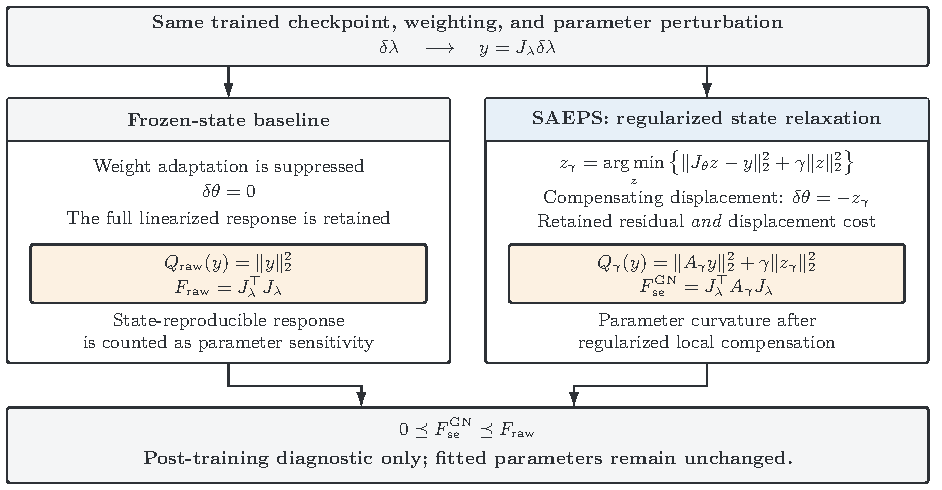
\includegraphics[width=.98\linewidth]{figures/fig01_geometry.pdf}
\caption{Frozen-state versus regularized state-relaxed curvature at the same trained checkpoint.
A parameter perturbation induces $y=J_\lambda\delta\lambda$.
Freezing $\delta\theta=0$ (left) assigns the entire quadratic response to $\Fraw$.
Allowing a compensating displacement $\delta\theta=-z_\gamma$ (right) evaluates the penalized energy $Q_\gamma=y^\top A_\gamma y=\|A_\gamma y\|_2^2+\gamma\|z_\gamma\|_2^2$ with $A_\gamma=I-J_\theta(J_\theta^\top J_\theta+\gamma I)^{-1}J_\theta^\top$, yielding $0\preceq\Fse\preceq\Fraw$ without updating the fitted parameters.}
\label{fig:geometry}
\end{figure}

To normalize across state scales, we parameterize $\gamma$ relative to the leading eigenvalue of $G_{\theta\theta}$ and track the effective state rank:
\begin{equation}
 \gamma=\alpha\lambda_{\max}(G_{\theta\theta}),\qquad
 r_{\rm eff}(\gamma)=\sum_i\frac{\sigma_i^2}{\sigma_i^2+\gamma}.
 \label{eq:gamma_scale}
\end{equation}
Because $G_{\theta\theta}$ is defined on the summed-loss scale of $\ell$, a mean-loss implementation using $\ell/m$ must divide both curvature blocks and $\gamma$ by $m$.
The scalar $\gamma$ is computed once at $(\theta_0,\lambda_0)$ and held fixed during differentiation and profiling.
As $\gamma\to\infty$, $\Fse$ approaches the frozen-state limit $\Fraw$; as $\gamma\to 0^+$ at fixed Jacobians, it approaches the variable-projection limit
\begin{equation}
 F^{\rm GN}_{\mathrm{VP},0}=\Jl^\top(I-\Jt\Jt^+)\Jl,
 \label{eq:fvp0}
\end{equation}
where $\Jt^+$ denotes the Moore--Penrose pseudoinverse.

\subsection{Exact error decomposition, dominance condition, and coordinate structure}
\label{sec:exact_reference}

To evaluate how accurately the Gauss--Newton reduction $\Fse$ captures exact local state relaxation, we define the anchor-regularized objective
\begin{equation}
 \mathcal L_\gamma(\theta,\lambda)=\ell(\theta,\lambda)+\tfrac\gamma2\|\theta-\theta_0\|_2^2,
 \label{eq:gamma_objective}
\end{equation}
assuming $\rbar$ is twice continuously differentiable with fixed weights, anchor $\theta_0$, and damping $\gamma$.

\medskip\noindent\textbf{Proposition 1 (Local profile curvature).}
Assume $\nabla_\theta\ell(\theta_0,\lambda_0)=0$ and $H_{\theta\theta}+\gamma I\succ 0$, where $H_{ab}=\nabla^2_{ab}\ell(\theta_0,\lambda_0)$.
Then a unique smooth state map $\theta_\gamma(\lambda)$ satisfies $\nabla_\theta\mathcal L_\gamma(\theta_\gamma(\lambda),\lambda)=0$ near $\lambda_0$, and the reduced objective $\Phi_\gamma(\lambda)=\mathcal L_\gamma(\theta_\gamma(\lambda),\lambda)$ has Hessian
\begin{equation}
 \nabla_\lambda^2\Phi_\gamma(\lambda_0)
 =\Hred
 =H_{\lambda\lambda}-H_{\lambda\theta}(H_{\theta\theta}+\gamma I)^{-1}H_{\theta\lambda}.
 \label{eq:exact_hred}
\end{equation}
\emph{Proof.}
By the implicit function theorem applied to $\nabla_\theta\mathcal L_\gamma=0$, $\mathrm d\theta_\gamma/\mathrm d\lambda=-(H_{\theta\theta}+\gamma I)^{-1}H_{\theta\lambda}$ at $\lambda_0$.
Differentiating $\Phi_\gamma(\lambda)$ twice and substituting this derivative yields Eq.~\eqref{eq:exact_hred}.\hfill$\square$

Notably, Proposition~1 requires only state stationarity $\nabla_\theta\ell=0$, not joint parameter stationarity $\nabla_\lambda\ell=0$.
Unlike classical hard-constrained PDE inverse problems~\cite{biros2005parallel,buithanh2013computational}---where an invertible discrete state-equation Jacobian permits undamped adjoint elimination---soft-constrained overparameterized PINNs frequently exhibit ill-conditioned $G_{\theta\theta}$ and indefinite or nearly singular unregularized state Hessians $H_{\theta\theta}$.
An arbitrary $\gamma>0$ does not automatically make an indefinite $H_{\theta\theta}+\gamma I$ positive definite unless $\gamma>-\lambda_{\min}(H_{\theta\theta})$; rather, selecting a sufficiently large finite $\gamma$ defines a well-posed local state-relaxed curvature while explicitly pricing compensating weight motion.

Define the exact fixed-state Hessian block and the exact and Gauss--Newton relaxation corrections as
\begin{align}
 \Hfix&=H_{\lambda\lambda},&
 \Cexact&=\Hfix-\Hred,&
 \Cgn&=\Fraw-\Fse.
 \label{eq:relaxation_defs}
\end{align}
Writing each exact Hessian block as $H_{ab}=G_{ab}+S_{ab}$ with residual-weighted second-order term $S_{ab}=\sum_i\bar r_i\nabla^2_{ab}\bar r_i$, the error of SAEPS relative to $\Hred$ obeys the exact identity
\begin{equation}
 \boxed{\Fse-\Hred
 =\underbrace{(\Fraw-\Hfix)}_{\Delta_{\rm GN,fix}}
 -\underbrace{(\Cgn-\Cexact)}_{\Delta_{\rm relax}}.}
 \label{eq:exact_error_identity}
\end{equation}
Equation~\eqref{eq:exact_error_identity} separates fixed-state Gauss--Newton truncation ($\Delta_{\rm GN,fix}$) from error in the relaxation correction ($\Delta_{\rm relax}$).
It also clarifies why a tiny relative error in $\Cgn$ can coexist with a larger relative error in $\Fse$: when $\Hred\ll\Hfix$, the reduced curvature is the difference of two large quantities.

\medskip\noindent\textbf{Corollary 1 (Sufficient dominance condition).}\label{cor:gain_condition}
For any fixed vector/matrix norm $\|\cdot\|$, define
\begin{equation}
 \chi=\frac{2\|\Delta_{\rm GN,fix}\|+\|\Delta_{\rm relax}\|}{\|\Cexact\|},
 \qquad \|\Cexact\|>0.
 \label{eq:gain_condition}
\end{equation}
If $\chi<1$, then $\|\Fse-\Hred\|<\|\Fraw-\Hred\|$.
\emph{Proof.}
By Eq.~\eqref{eq:exact_error_identity} and the triangle inequality, $\|\Fse-\Hred\|\le\|\Delta_{\rm GN,fix}\|+\|\Delta_{\rm relax}\|$, whereas $\|\Fraw-\Hred\|=\|\Delta_{\rm GN,fix}+\Cexact\|\ge\|\Cexact\|-\|\Delta_{\rm GN,fix}\|$.
Rearranging $\chi<1$ gives the claim.\hfill$\square$

Here $\|\cdot\|_2$ denotes the Euclidean/spectral norm and $\|\cdot\|_F$ the Frobenius norm, applied consistently across all terms in Eq.~\eqref{eq:gain_condition}.
Corollary~1 explains retroactively why SAEPS outperforms $\Fraw$ whenever omitted state relaxation dominates second-order residual terms.

\paragraph{Coordinate and non-affine structure.}
\label{sec:coordinate_identity}
In many inverse PDEs, the residual is affine in a positive physical coefficient $a$:
\begin{equation}
 \rbar(\theta,a)=c(\theta)+a\,b(\theta),\qquad a=e^\lambda.
 \label{eq:affine_parameter}
\end{equation}
Under parameter-independent weights, Eq.~\eqref{eq:affine_parameter} implies
\begin{equation}
 H_{aa}=G_{aa},\qquad H_{\lambda\lambda}-G_{\lambda\lambda}=\partial_\lambda\ell,
 \label{eq:score_truncation}
\end{equation}
with $\operatorname{diag}(\nabla_\lambda\ell)$ for componentwise log-transformed multi-parameter vectors.
More generally, changing from $a$ to $\lambda=\log a$ transforms the exact and Gauss--Newton reduced curvatures as
\begin{equation}
 H_{{\rm red},\lambda}=a^2H_{{\rm red},a}+a\,\partial_a\ell,\qquad
 F_{{\rm se},\lambda}^{\rm GN}=a^2F_{{\rm se},a}^{\rm GN}.
 \label{eq:coordinate_change}
\end{equation}
Thus nonzero fixed-state truncation $H_{\lambda\lambda}-G_{\lambda\lambda}$ arises even for parameter-affine PDEs whenever $\partial_\lambda\ell\ne 0$ after state-only refinement, whereas genuinely non-affine physical parameters contribute an additional second-order term $a^2\sum_i\bar r_i\partial_{aa}\bar r_i$.
Similarly, under a linear state reparameterization $\theta-\theta_0=Tz$, invariance of $\mathcal L_\gamma$ requires transforming the Euclidean penalty to $\gamma z^\top T^\top Tz/2$; spectral scaling alone does not confer general coordinate invariance.

\subsection{Matrix-free evaluation and a posteriori energy bound}
\label{sec:matrix_free}

Evaluating $\Fse$ requires only Jacobian--vector products ($\Jt v$) and vector--Jacobian products ($\Jt^\top w$) to solve $MZ=\Jt^\top Y$ with $Y=\Jl\in\RR^{m\times p}$, avoiding explicit assembly of $\Jt\in\RR^{m\times n_\theta}$.
For an approximate solution $\widehat Z\approx M^{-1}\Jt^\top Y$, define the normal-equation residual and energy-form curvature estimate
\begin{equation}
 R=M\widehat Z-\Jt^\top Y,\qquad
 \widehat F_E=(Y-\Jt\widehat Z)^\top(Y-\Jt\widehat Z)+\gamma\widehat Z^\top\widehat Z.
 \label{eq:approximate_energy}
\end{equation}
Unlike direct subtraction $Y^\top Y - Y^\top\Jt\widehat Z$, the energy form $\widehat F_E$ preserves positive semidefiniteness by construction and admits an exact algebraic error bound.

\medskip\noindent\textbf{Proposition 2 (A posteriori linear-solve error bound).}
In exact arithmetic,
\begin{equation}
 \widehat F_E-\Fse=R^\top M^{-1}R,\qquad
 0\preceq\widehat F_E-\Fse\preceq\gamma^{-1}R^\top R.
 \label{eq:energy_certificate}
\end{equation}
\emph{Proof.}
Write $\widehat Z=Z_\star+E$ where $MZ_\star=\Jt^\top Y$.
Expanding Eq.~\eqref{eq:approximate_energy} cancels the linear cross terms via $M Z_\star=\Jt^\top Y$, leaving $\widehat F_E-\Fse=E^\top M E=R^\top M^{-1}R$.
Since $M=\Jt^\top\Jt+\gamma I\succeq\gamma I$, the upper bound follows.\hfill$\square$

Consequently, $\|R\|_2^2/\gamma$ bounds the spectral-norm linear-solve error using only quantities available after the iterative solve.
Algorithm~\ref{alg:saeps} summarizes the complete matrix-free evaluation and audit procedure.

\begin{algorithm}[!htbp]
\centering
\small
\caption{Matrix-free SAEPS curvature evaluation and a posteriori energy audit.}
\label{alg:saeps}
\begin{tabular}{@{}p{.96\linewidth}@{}}
\toprule
\textbf{Input:} Trained checkpoint $(\theta_0,\lambda_0)$, weighted residual map $\rbar(\theta,\lambda)$, dimensionless damping $\alpha>0$, solver tolerance $\tau_{\rm solve}$.\\
\textbf{Output:} Frozen curvature $\Fraw$, state-relaxed curvature $\widehat F_E$, solve-error bound $\epsilon_{\rm solve}$, retained ratio $\eta$.\\
\midrule
1.\ Form parameter Jacobian $Y=\Jl\in\RR^{m\times p}$ via forward-mode differentiation and compute $\Fraw=Y^\top Y$.\\
2.\ Estimate $\lambda_{\max}(G_{\theta\theta})$ via power iteration using matrix-free products $v\mapsto\Jt^\top(\Jt v)$; set $\gamma=\alpha\lambda_{\max}(G_{\theta\theta})$.\\
3.\ For each column $y_k$ of $Y$ ($k=1,\dots,p$), solve $(\Jt^\top\Jt+\gamma I)\hat z_k=\Jt^\top y_k$ to relative residual $\le\tau_{\rm solve}$ using matrix-free CG or scaled augmented LSQR; assemble $\widehat Z=[\hat z_1,\dots,\hat z_p]$.\\
4.\ Evaluate normal residual $R=(\Jt^\top\Jt+\gamma I)\widehat Z-\Jt^\top Y$ and energy curvature $\widehat F_E=(Y-\Jt\widehat Z)^\top(Y-\Jt\widehat Z)+\gamma\widehat Z^\top\widehat Z$.\\
5.\ Compute a posteriori spectral error bound $\epsilon_{\rm solve}=\|R\|_2^2/\gamma$ and per-coordinate retained ratios $\eta_k=(\widehat F_E)_{kk}/(\Fraw)_{kk}$.\\
\bottomrule
\end{tabular}
\end{algorithm}

\section{Experimental design and evaluation protocol}
\label{sec:numerical_setup}

Our numerical study tests four questions aligned with Sections~\ref{sec:introduction}--\ref{sec:method}: (i) how severely $\Fraw$ overestimates $\Hred$ across affine, non-affine, and coupled inverse PDEs; (ii) whether the error budget, dominance condition, and undamped-limit audits explain the observed gains; (iii) how accuracy and solver cost behave as state dimension grows; and (iv) how closely local Schur curvature matches finite-step nonlinear profile differences.

\subsection{Benchmark suite}
\label{sec:benchmarks}

All scalar PDEs are posed on $x\in[0,1]$, $t\in[0,0.4]$ with periodic boundary conditions matching solution values and spatial derivatives, and all physical parameters are inferred in logarithmic coordinates.
Table~\ref{tab:design} summarizes the five evaluation cohorts.

\begin{table}[!htbp]
\centering
\caption{Benchmark cohorts. Trained accuracy studies span $n_\theta=33$--$337$, whereas large-scale operator feasibility uses a separate function-preserving expansion.}
\label{tab:design}
\small
\begin{tabular}{lcll}
\toprule
Problem & $p$ & Network / $n_\theta$ & Planned evaluation\\
\midrule
Burgers & 1 & $2$--$16$--$1$ / 65 & 15 checkpoints\\
Allen--Cahn & 1 & $2$--$8$--$1$ / 33 & 10 checkpoints\\
Saturation (non-affine) & 1 & $2$--$16$--$1$ / 65 & 24 held-out fits (6 data seeds)\\
Architecture scaling (Saturation) & 1 & 65, 129, 337 & 6 paired fits per size\\
Coupled reaction--diffusion & 2 & Two width-6 nets / 50 & 10 checkpoints\\
\bottomrule
\end{tabular}
\end{table}

\paragraph{Affine scalar PDEs.}
We first evaluate Burgers and Allen--Cahn inverse problems:
\begin{align}
 u_t+uu_x&=\mu u_{xx}, & u(x,0)&=\sin(2\pi x), & \mu^\star&=0.05,\;\mu_{\rm init}=0.08,\label{eq:burgers_setup}\\
 u_t&=0.01u_{xx}+\rho(u-u^3), & u(x,0)&=0.5\sin(2\pi x), & \rho^\star&=2.0,\;\rho_{\rm init}=1.4.\label{eq:allen_setup}
\end{align}
Reference trajectories are generated independently using a finite-difference spatial discretization ($128$ grid points) with fourth-order Runge--Kutta time integration ($2000$ steps).

\paragraph{Non-affine saturation PDE.}
To test parameter nonlinearity beyond Eq.~\eqref{eq:affine_parameter}, we infer the saturation coefficient $\kappa$ ($\lambda=\log\kappa$, $\kappa^\star=1.2$, $\kappa_{\rm init}=0.8$) in
\begin{equation}
 u_t=D u_{xx}+\rho\frac{u}{1+\kappa u}+f(x,t),\qquad D=0.01,\quad \rho=1,
 \label{eq:saturation_system}
\end{equation}
with manufactured solution $u^\star(x,t)=1+0.2e^{-t}\cos(2\pi x)+0.1e^{-2t}\sin(4\pi x)$.
The source $f$ is evaluated once at $\kappa^\star$ and held fixed during inference to isolate parameter non-affinity from forcing misspecification.
A softplus output layer shifted by $0.05$ guarantees state positivity, with all network derivatives propagated through the transformation.
Observations are tested at noise levels $0$ and $0.02\times\operatorname{std}(u^\star)$ using shared sampling locations and standard-normal draws across two initializations per data seed, yielding $8$ development fits ($2$ seeds) and $24$ held-out fits ($6$ seeds).

\paragraph{Coupled two-parameter PDE.}
For joint multi-parameter geometry, we infer $(\log a,\log b)$ in a two-field reaction--diffusion system:
\begin{align}
 u_t&=0.03u_{xx}-au+bv+f_u, & v_t&=0.02v_{xx}+au-bv+f_v,
 \label{eq:coupled_system}
\end{align}
with true values $(0.8,0.75)$, initial estimates $(0.6,0.95)$, Dirichlet boundary data, and fixed manufactured sources (details in the Supplementary Material).
Two width-6 $\tanh$ networks represent $u$ and $v$, giving $n_\theta=50$ state parameters jointly.

\subsection{Training, state refinement, and numerical validity}
\label{sec:training_protocol}

Each scalar residual vector stacks $96$ PDE collocation points, $128$ observations, $48$ initial points, and $96$ periodic boundary entries ($m=368$), weighted by fixed positive block weights $w_b=(5,10,10,2)$ across training, Hessian assembly, and SAEPS evaluation.
The coupled problem stacks $m=736$ residual entries.
Training minimizes the mean loss $\ell/m$, whereas curvature matrices and $\gamma$ are reported on the summed scale $\ell$ in \texttt{float64} precision at prespecified nominal damping $\alpha=10^{-8}$.

For Burgers and Allen--Cahn, training runs $1600$ Adam steps (learning rate $3\times10^{-3}$) followed by up to $300$ joint L-BFGS iterations.
To satisfy the state-stationarity premise of Proposition~1 for exact-reference validation, the fitted physical parameter $\lambda_0$ is held fixed while only the neural state $\theta$ is refined.
For the saturation benchmark, joint training uses $3000$ Adam steps ($10^{-3}$) and up to $1000$ L-BFGS iterations, followed by fixed-$\lambda$ state refinement capped at $100{,}000$ iterations (increased from $30{,}000$ during development after observing individual error changes up to $14.2\%$, then frozen before held-out execution).

Every checkpoint is audited before entering exact-reference comparisons using
\begin{equation}
 g_\theta^{\rm norm}=\frac{\|\nabla_\theta(\ell/m)\|_2}{\max(\|\theta\|_2,1)},\qquad
 s_\theta=\frac{\|\Jt^\top\rbar\|_2}{\|\Jt\|_F\|\rbar\|_2+\epsilon_{\rm mach}}.
 \label{eq:stationarity_definitions}
\end{equation}
State refinement targets $g_\theta^{\rm norm}\le 10^{-6}$, and final center validity requires $g_\theta^{\rm norm}<10^{-4}$, $s_\theta<10^{-4}$, Hessian symmetry within $10^{-8}$, positive definiteness of $H_{\theta\theta}+\gamma I$, and verified linear-solve residuals $\le 10^{-8}$ (complete threshold tables appear in the Supplementary Material).
Invalid checkpoints lack a valid positive-definite reference $\Hred$; they are retained in planned cohort counts rather than silently discarded.

\subsection{Error metrics and statistical protocol}
\label{sec:metrics}

All scalar methods are compared at identical checkpoints, weights, coordinates, anchors, and damping.
Here $\Fraw$ serves as the same-checkpoint coupling-ablation baseline and $\Hred$ as the matched-damping exact reference; training-time decoupling~\cite{uriarte2025least,zhang2026bilo} and second-order optimizers~\cite{muller2023engd} alter the fitted checkpoint itself and are therefore complementary to, rather than competing with, post-training curvature correction.
Relative curvature errors and component errors are normalized consistently by $|\Hred|+\varepsilon$ ($\varepsilon=10^{-8}$):
\begin{align}
 \Eraw&=\frac{|\Fraw-\Hred|}{|\Hred|+\varepsilon}, &
 \Esa&=\frac{|\Fse-\Hred|}{|\Hred|+\varepsilon}, \label{eq:scalar_errors}\\
 E_{\rm fix}&=\frac{|\Hfix-\Hred|}{|\Hred|+\varepsilon}, &
 E_{\rm GN,fix}&=\frac{|\Fraw-\Hfix|}{|\Hred|+\varepsilon}, \label{eq:fixed_state_exact_error}
\end{align}
while accuracy of the relaxation correction itself uses its own scale:
\begin{equation}
 E_{\rm relax}=\frac{|\Cgn-\Cexact|}{|\Cexact|+\varepsilon}.
 \label{eq:relaxation_error}
\end{equation}
The coupled two-parameter benchmark uses a stabilized raw-matrix whitening metric (Supplementary Material, Section~S3).

On each comparable unit, paired improvement is defined as $D=\Eraw-\Esa$ and tested with an exact one-sided sign test under $H_0:\Pr(D>0\mid D\ne 0)=1/2$ (no ties occur in any scalar cohort; all $p$-values are unadjusted and conditional on numerical validity, without assuming ignorable missingness).
For Burgers and Allen--Cahn, each valid checkpoint is an independent unit.
For saturation, the data seed is the independent unit; the four dependent fits per seed (two initializations $\times$ two noise levels) are summarized by their seed median (a post-hoc cross-noise pooling rule), alongside individual-fit and within-noise summaries in the Supplementary Material.
Exact fixed-state blocks for the Burgers and Allen--Cahn decompositions reproduce their primary scalar curvature records to within $3.51\times10^{-16}$ relative discrepancy.

\section{Results}
\label{sec:results}

\subsection{Curvature correction across affine, non-affine, and coupled benchmarks}
\label{sec:scalar_results}

At the prespecified damping $\alpha=10^{-8}$, regularized state elimination reduces frozen-state curvature error by one to four orders of magnitude on every valid checkpoint across all tested PDEs (Fig.~\ref{fig:accuracy} and Table~\ref{tab:main_results}).
On the affine scalar benchmarks, $12/15$ Burgers checkpoints and $9/10$ Allen--Cahn checkpoints pass the numerical center checks, and every valid checkpoint favors SAEPS.
Median relative curvature error drops from $27.73$ to $0.0750$ on Burgers ($370$-fold ratio of medians, $335$-fold median of paired ratios, $p=2.44\times10^{-4}$) and from $20.37$ to $0.2786$ on Allen--Cahn ($73$-fold ratio of medians, $79$-fold median of paired ratios, $p=1.95\times10^{-3}$).
The remaining errors ($7.50\%$ and $27.86\%$) confirm that SAEPS removes the bulk of frozen-state bias without claiming exact Hessian recovery.

\begin{figure}[!htbp]
\centering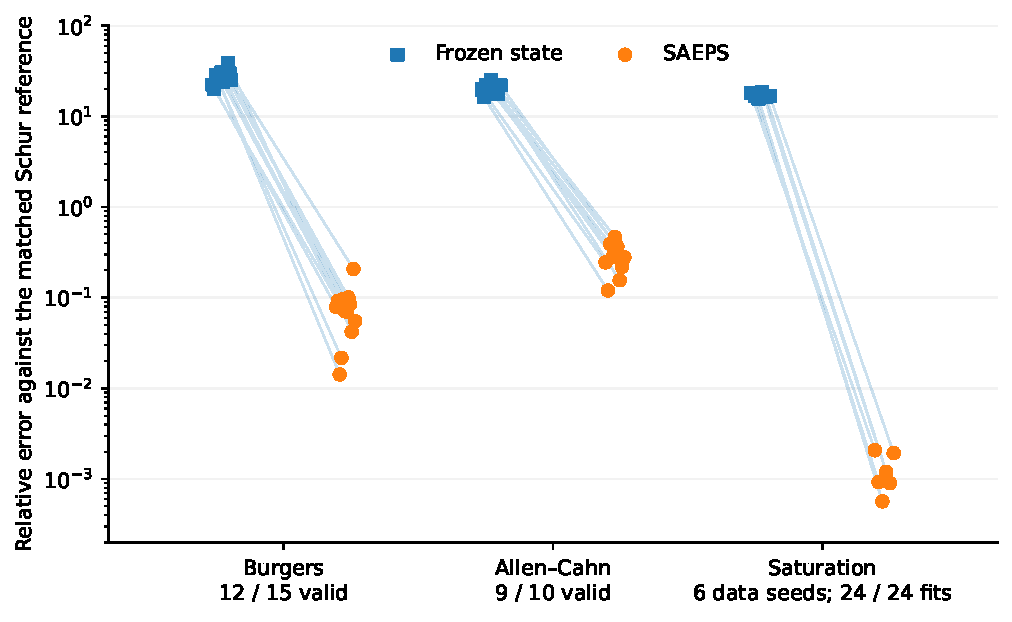
\includegraphics[width=.98\linewidth]{figures/fig02_paired_accuracy.pdf}
\caption{Paired relative curvature errors across the three scalar benchmarks at $\alpha=10^{-8}$.
Each line connects frozen-state ($\Eraw$) and state-relaxed ($\Esa$) errors at the same valid checkpoint.
Saturation points represent the six held-out data-seed medians (each pooling four dependent fits); planned denominators are preserved in all labels and in Table~\ref{tab:main_results}.}
\label{fig:accuracy}
\end{figure}
\begin{table}[!htbp]
\centering
\caption{Primary scalar curvature comparison against exact finite-$\gamma$ reduced-Hessian references at $\alpha=10^{-8}$. Bold entries denote the lower median error per benchmark.}
\label{tab:main_results}
\small
\setlength{\tabcolsep}{4pt}
\begin{tabular}{lcc S[table-format=2.4] S[table-format=1.6] S[table-format=1.4e-1,scientific-notation=true]}
\toprule
{Problem} & {Valid/planned} & {Units} & {Median $E_{\rm raw}$} & {Median $E_{\rm SAEPS}$} & {$p$} \\
\midrule
Burgers & 12/15 & 12 & 27.7268 & \bfseries 0.0750 & 2.44e-04 \\
Allen--Cahn & 9/10 & 9 & 20.3728 & \bfseries 0.2786 & 1.95e-03 \\
Saturation & 24/24 fits & 6 seeds & 16.8165 & \bfseries 0.001060 & 1.5625e-02 \\
\bottomrule
\end{tabular}
\par\vspace{3pt}\begin{minipage}{.98\linewidth}\footnotesize Errors are dimensionless relative discrepancies against $\Hred$. Burgers and Allen--Cahn units are valid checkpoints; saturation units are six held-out data-seed medians (each pooling four dependent fits across two initializations and two noise levels). All $24$ saturation fits improve individually. Values of $p$ are unadjusted, exact one-sided sign tests under $H_0:\Pr(D>0\mid D\ne0)=1/2$ with no ties; saturation cross-noise pooling is post hoc. Invalid checkpoints remain in planned counts and are excluded from numerical-error summaries.\end{minipage}
\end{table}


Beyond parameter-affine residuals, SAEPS retains its advantage on the genuinely non-affine saturation PDE.
All $24/24$ held-out fits across six data seeds admit the exact reduction and outperform $\Fraw$.
At the independent data-seed level, $6/6$ seeds favor SAEPS ($p=1.56\times10^{-2}$), lowering median relative error from $\SaturationRaw$ to $\SaturationError$ ($\SaturationPercent\%$; individual-fit median $\SaturationFitError$).
The seed-level paired improvement has median $\SaturationDMedian$ and interquartile range $[\SaturationDLower,\SaturationDUpper]$.
Automatic differentiation confirms the exact non-affine residual-Hessian identity
\begin{equation}
 H_{\lambda\lambda}-G_{\lambda\lambda}-g_\lambda
 =\kappa^2\sum_i\bar r_i\,\partial_{\kappa\kappa}\bar r_i,
 \qquad
 r_{\kappa\kappa}=-2\rho\frac{u^3}{(1+\kappa u)^3},
 \label{eq:nonaffine_identity}
\end{equation}
verifying that physical non-affinity contributes distinctly from the log-coordinate gradient term $g_\lambda=\partial_\lambda\ell$, though the second-order term remains small at these well-fitted centers.

Consistent directional gains also appear in two auxiliary cohorts.
In the coupled two-parameter reaction--diffusion system, $8/10$ checkpoints pass the numerical validity checks, and all $8$ favor SAEPS under the whitened matrix metric; because $8/10$ falls below the prespecified $9/10$ availability gate, we report this as directional rather than confirmatory matrix evidence.
Across $15$ designated noise-and-sparsity stress anchors on Burgers, $14/15$ pass validity and all $14$ favor SAEPS, reducing median error from $38.13$ to $0.0879$ (full stress grids and failure breakdowns appear in the Supplementary Material).

\subsection{Mechanism verification: error budget, dominance condition, and damping audits}
\label{sec:mechanism_results}

Table~\ref{tab:mechanism} and Fig.~\ref{fig:mechanism} apply the exact decomposition of Eq.~\eqref{eq:exact_error_identity} to explain why SAEPS achieves orders-of-magnitude gains.
Across all three scalar PDEs, omitted state relaxation ($E_{\rm fix}$) dominates fixed-state Gauss--Newton truncation ($E_{\rm GN,fix}$) by roughly two to four orders of magnitude: $27.75$ versus $0.1563$ on Burgers, $19.95$ versus $0.2903$ on Allen--Cahn, and $16.80$ versus $\SaturationGNError$ on saturation.
Moreover, SAEPS recovers the exact relaxation correction $\Cexact$ to sub-percent median precision across every benchmark, with median correction errors $E_{\rm relax}$ of $0.31\%$ (Burgers), $0.23\%$ (Allen--Cahn), and $1.26\times10^{-3}\%$ (saturation).

\begin{table}[!htbp]
\centering
\caption{The state-freezing term dominates the observed error budgets.}
\label{tab:mechanism}
\small
\setlength{\tabcolsep}{4pt}
\begin{tabular}{l S[table-format=2.4] S[table-format=1.6] S[table-format=1.6] S[table-format=1.3e-1,scientific-notation=true]}
\toprule
{Problem} & {$E_{\rm fix}$} & {$E_{\rm GN,fix}$} & {$E_{\rm SAEPS}$} & {$E_{\rm relax}$} \\
\midrule
Burgers & 27.75 & 0.1563 & 0.07503 & 0.00308 \\
Allen--Cahn & 19.95 & 0.2903 & 0.2786 & 0.00234 \\
Saturation & 16.8 & 0.001181 & 0.001247 & 1.259e-05 \\
\bottomrule
\end{tabular}
\par\vspace{3pt}\begin{minipage}{.98\linewidth}\footnotesize Entries are medians over 12, 9, and 24 accepted fits, respectively. The first three errors share the reduced-curvature denominator. The correction error $E_{\rm relax}$ uses $|C_{\rm relax}^{\rm exact}|+10^{-8}$. Historical decomposition values retain their archived precision; the two normalizations are not interchangeable.\end{minipage}
\end{table}

\begin{figure}[!htbp]
\centering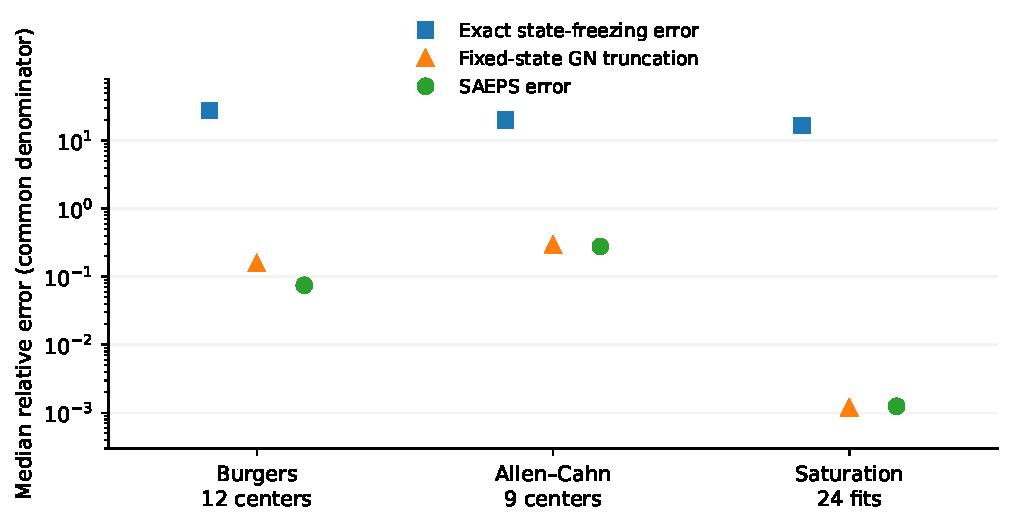
\includegraphics[width=.95\linewidth]{figures/fig03_error_mechanisms.pdf}
\caption{Error-budget decomposition separating omitted state relaxation ($E_{\rm fix}$) from fixed-state Gauss--Newton truncation ($E_{\rm GN,fix}$) and remaining SAEPS error ($\Esa$).
All plotted quantities share the reduced-curvature denominator $|\Hred|+10^{-8}$; saturation medians pool all $24$ held-out fits.
Correction-relative errors $E_{\rm relax}$ use $|\Cexact|+10^{-8}$ and are listed in Table~\ref{tab:mechanism}.}
\label{fig:mechanism}
\end{figure}

This budget also explains the gap between sub-percent median correction accuracy and the larger final curvature errors on Burgers ($7.50\%$) and Allen--Cahn ($27.86\%$): because $\Hred$ is more than an order of magnitude smaller than $\Hfix$, residual truncation $\Delta_{\rm GN,fix}$ is amplified when normalized by $|\Hred|$.
Evaluating Corollary~1 across all $39$ valid scalar centers confirms that every center satisfies $\chi<1$: Burgers ($12/12$, $\chi\in[0.0081,0.0260]$, median $0.0153$), Allen--Cahn ($9/9$, $\chi\in[0.0229,0.0457]$, median $0.0329$), and the $18$ saturation architecture centers ($6$ shared base fits plus $12$ wider/deeper fits, $\max\chi=\GainRatioMaximum$).

\paragraph{Undamped-limit ill-conditioning and finite-damping trade-off.}
Two additional audits documented in the Supplementary Material clarify the role of finite damping $\gamma>0$.
First, across the $21$ valid Burgers and Allen--Cahn checkpoints, the resolved eigen-subspaces of $G_{\theta\theta}=\Jt^\top\Jt$ are severely ill-conditioned, with median condition numbers of $2.70\times 10^{13}$ on Burgers (numerical rank $60/65$) and $7.37\times 10^{12}$ on Allen--Cahn (rank $32/33$).
None of the $21$ checkpoints ($0/12$ on Burgers, $0/9$ on Allen--Cahn) passes the prespecified undamped positive-definiteness threshold for $H_{\theta\theta}$ ($19$ exhibit negative minimum eigenvalues and $2$ have positive eigenvalues below tolerance), while the formal truncated-SVD pseudoinverse $F^{\rm GN}_{\mathrm{VP},0}$ varies by up to $48.5\%$ on Burgers and $23.4\%$ on Allen--Cahn with cutoff choice.
Second, sweeping $\alpha\in[10^{-10},10^2]$ across six fixed Burgers and Allen--Cahn centers shows that only $2/6$ centers resolve numerically at $\alpha=10^{-10}$, whereas all $6/6$ resolve from $\alpha=10^{-8}$ upward; median retained sensitivity increases monotonically from $0.0483$ ($r_{\rm eff}=35.78$) at $\alpha=10^{-8}$ to $0.5798$ ($r_{\rm eff}=6.58$) at $\alpha=10^{-2}$ and $0.9996$ ($r_{\rm eff}=0.015$) at $\alpha=100$, recovering $\Fraw$.
Although median $\Esa(\alpha)$ falls from $0.1630$ at $\alpha=10^{-8}$ to $0.0185$ at $\alpha=10^{-2}$ (Supplementary Material, Table~S14), errors at different $\alpha$ are not directly comparable because changing $\gamma$ shifts the reference target $\Hred$ toward $\Fraw$; $\alpha=10^{-8}$ was prespecified before confirmation rather than selected from this sweep.

\subsection{State-dimension scaling and computational cost}
\label{sec:scaling_and_cost}

We next examine whether the curvature advantage persists in larger trained state spaces and quantify the computational trade-off among dense and matrix-free solvers.

\paragraph{Trained architecture scaling.}
Holding data seeds, initializations, and observation noise ($0.02$) fixed on the saturation problem, we train paired networks with $n_\theta=65$, $129$, and $337$ state parameters ($6$ fits per size).
Every fit admits the exact reduction and outperforms $\Fraw$ by roughly four orders of magnitude (Table~\ref{tab:architecture} and Fig.~\ref{fig:architecture}), with median SAEPS errors decreasing from $\BaseError$ ($n_\theta=65$) to $\WideError$ ($129$) and $\DeepError$ ($337$).
Individual paired trajectories show that improvement is not strictly monotone for every seed--architecture pair (two width-$32$ fits have slightly higher $\Esa$ than their width-$16$ counterparts), yet all $18/18$ fits remain well below $\Fraw\approx 17$.
At $n_\theta=337$, the largest dense-Hessian versus HVP discrepancy across tested directions is $1.54\times10^{-15}$, verifying derivative assembly.
(On the Burgers stress suite, by contrast, width-$32$ networks yielded $0/5$ valid state centers under the original budget, underscoring that larger state spaces remain sensitive to center-convergence availability.)

\begin{table}[!htbp]
\centering
\caption{Paired curvature errors across trained architectures on the saturation problem. Bold entries denote the lower median error per architecture.}
\label{tab:architecture}
\small
\setlength{\tabcolsep}{4pt}
\begin{tabular}{l S[table-format=3.0] c S[table-format=2.4] S[table-format=1.3e-1,scientific-notation=true] S[table-format=1.6]}
\toprule
{Architecture} & {$n_\theta$} & {Valid} & {Median $E_{\rm raw}$} & {Median $E_{\rm SAEPS}$} & {Coefficient error} \\
\midrule
2--16--1 & 65 & 6/6 & 16.797 & \bfseries 0.0009224 & 0.01302 \\
2--32--1 & 129 & 6/6 & 16.931 & \bfseries 0.0006087 & 0.007905 \\
2--16--16--1 & 337 & 6/6 & 17.266 & \bfseries 0.0004322 & 0.004592 \\
\bottomrule
\end{tabular}
\par\vspace{3pt}\begin{minipage}{.98\linewidth}\footnotesize Each architecture evaluates three data seeds and two initializations at observation noise $0.02$. The six base ($n_\theta=65$) fits are shared with the main saturation cohort; twelve wider and deeper fits are additional. The rightmost column reports the median parameter error $|\widehat\kappa-\kappa^\star|/\kappa^\star$ of the underlying PINN fits, which post-training SAEPS leaves unchanged.\end{minipage}
\end{table}

\begin{figure}[!htbp]
\centering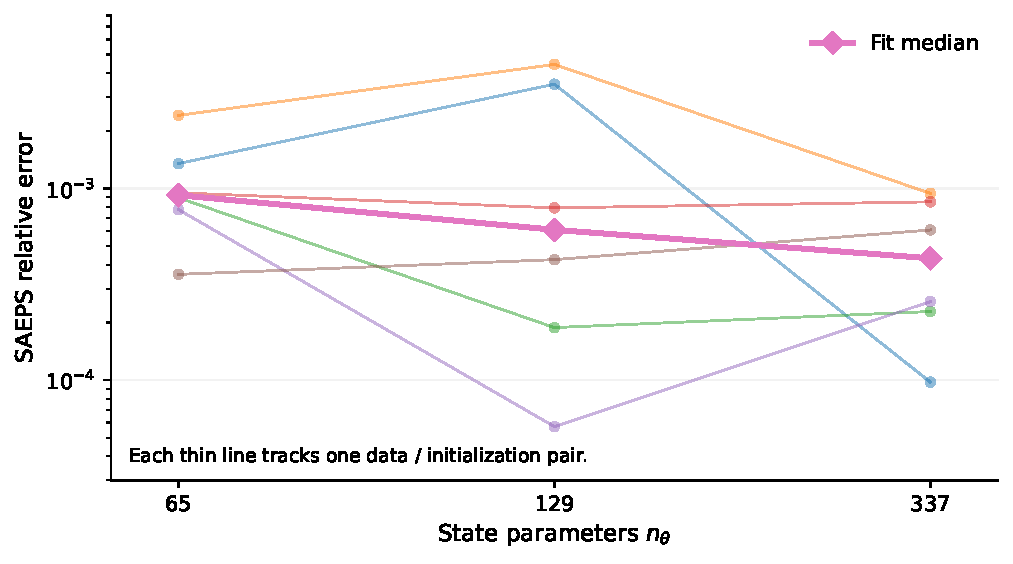
\includegraphics[width=.98\linewidth]{figures/fig04_architecture_pairs.pdf}
\caption{Paired curvature errors across trained architectures ($n_\theta=65, 129, 337$) on the saturation problem, plotted alongside the frozen-state baseline ($\Eraw$) on a common logarithmic scale.
Thin lines connect identical data seeds and initializations across network sizes; thick curves show six-fit medians.}
\label{fig:architecture}
\end{figure}

\paragraph{Matched-damping solver cost and large-scale operator feasibility.}
To separate solver efficiency from numerical agreement, we benchmark dense Cholesky factorization, matrix-free CG, and scaled augmented LSQR at identical damping across four scales ($\alpha\in\{10^{-8},10^{-6},10^{-4},10^{-2}\}$), two coupled checkpoints ($n_\theta=50$, $p=2$, $m=736$), and three timed repeats following a discarded warm-up with zero initial guesses.
All $72$ evaluations pass their verification checks (Fig.~\ref{fig:cost}).
Dense factorization and CG solve two parameter-column right-hand sides, whereas the scaled-LSQR implementation invokes three polarized residual solves.
At $n_\theta=50$, dense Cholesky is fastest across all damping scales ($\sim 10^{-4}\text{ s}$).
For matrix-free CG, solve time depends strongly on damping through Krylov conditioning: at $\alpha=10^{-2}$, CG takes only $0.60\text{ s}$ and $0.54\text{ s}$ at the two checkpoints, rising to $10.63\text{ s}$ and $5.23\text{ s}$ at weak damping $\alpha=10^{-8}$ as iteration counts grow across both right-hand sides (with Python autograd product overhead dominating per-iteration cost at $n_\theta=50$).
At $\alpha=10^{-8}$, scaled LSQR takes $143.27\text{ s}$ and $134.63\text{ s}$, attaining dense-reference discrepancies of $1.19\times10^{-12}$ and $1.98\times10^{-11}$ compared with $2.99\times10^{-8}$ and $4.82\times10^{-8}$ for CG; both iterative solvers exceed the $10^{-6}$ algebraic agreement target.

\begin{figure}[!htbp]
\centering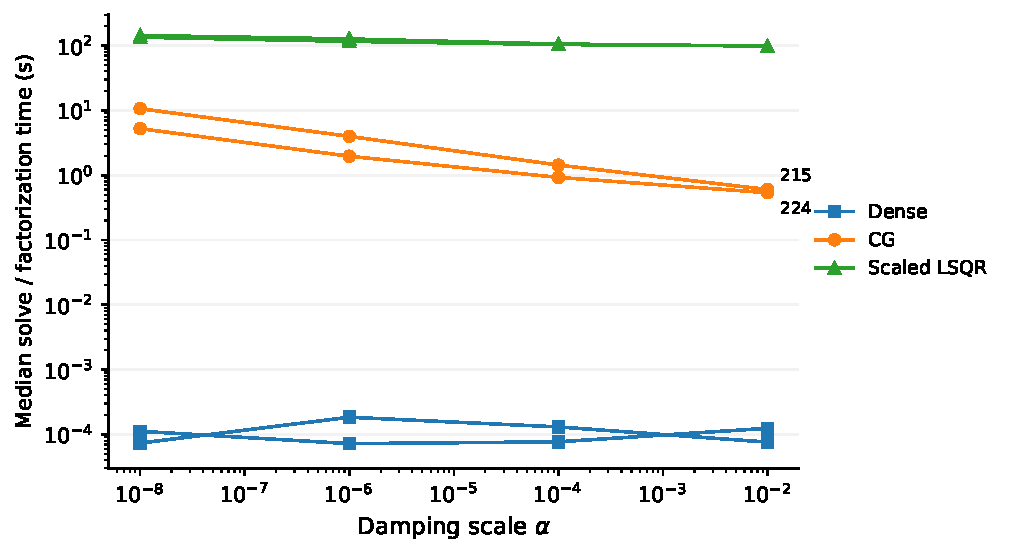
\includegraphics[width=.98\linewidth]{figures/fig05a_matched_cost.pdf}
\caption{Matched-damping wall-clock solve times across dense Cholesky, matrix-free CG, and scaled augmented LSQR at two coupled checkpoints ($n_\theta=50$, $p=2$, $m=736$).
Colors and markers distinguish solvers; solid and dashed lines distinguish the two checkpoints.
Each point is a three-repeat median excluding shared Jacobian preparation; complete timing ledgers and agreement curves appear in the Supplementary Material.}
\label{fig:cost}
\end{figure}

While explicit factorization is preferable for small networks, matrix-free products avoid storing $\Jt\in\RR^{m\times n_\theta}$ at scale.
In a separate operator-feasibility test using function-preserving width expansion at $\alpha=10^{-2}$ up to $n_\theta=100{,}001$ state parameters and $m=3413$ residuals, all $27/27$ timing runs pass verified residual checks; the largest grid requires $62.83\text{ s}$ of shared setup and $40.97\text{ s}$ of median CG iteration time (a $\sim 70\times$ increase over the matched $\alpha=10^{-2}$ solve time of $0.54$--$0.60\text{ s}$ at $n_\theta=50, m=736$).
The exact-arithmetic energy bound of Proposition~2 is verified separately in algebraic unit tests (Supplementary Material).

\subsection{Finite-perturbation profile resolution}
\label{sec:profile_resolution}

Because $\Hred$ is an infinitesimal local derivative, we test whether it agrees with finite-displacement state reoptimization under fixed anchor $\theta_0$ and damping $\gamma$.
Along a unit parameter direction $v$, the symmetric finite difference
\begin{equation}
 D_\gamma(h;v)=\frac{\Phi_\gamma(\lambda_0+hv)-2\Phi_\gamma(\lambda_0)+\Phi_\gamma(\lambda_0-hv)}{h^2}
 \label{eq:profile_difference}
\end{equation}
cancels first-order parameter gradients and targets $v^\top\Hred v$ as $h\to 0$ (distinct from likelihood-ratio profiling for statistical identifiability~\cite{raue2009structural}).

Across three saturation data seeds and seven step sizes ($21$ symmetric differences total; Fig.~\ref{fig:profile}), all $21$ pairs pass the branch-displacement comparability check and $20/21$ agree with $\Hred$ within $10\%$.
However, $0/21$ branch pairs reach the strictest state-gradient tolerance at any step size, and only $5/126$ individual branch refinements satisfy their assigned graded tolerance.
At the smallest steps, residual optimization error is amplified by $h^{-2}$, preventing strict multiscale convergence.
This mirrors a separate five-case profile benchmark in which only $1/5$ cases met both small-radius consistency gates (Supplementary Material).
Accordingly, these results establish intermediate-radius numerical agreement ($20/21$ within $10\%$) alongside unresolved strict state convergence ($0/21$ at the strictest gate), rather than nonlinear profile equivalence.

\begin{figure}[!htbp]
\centering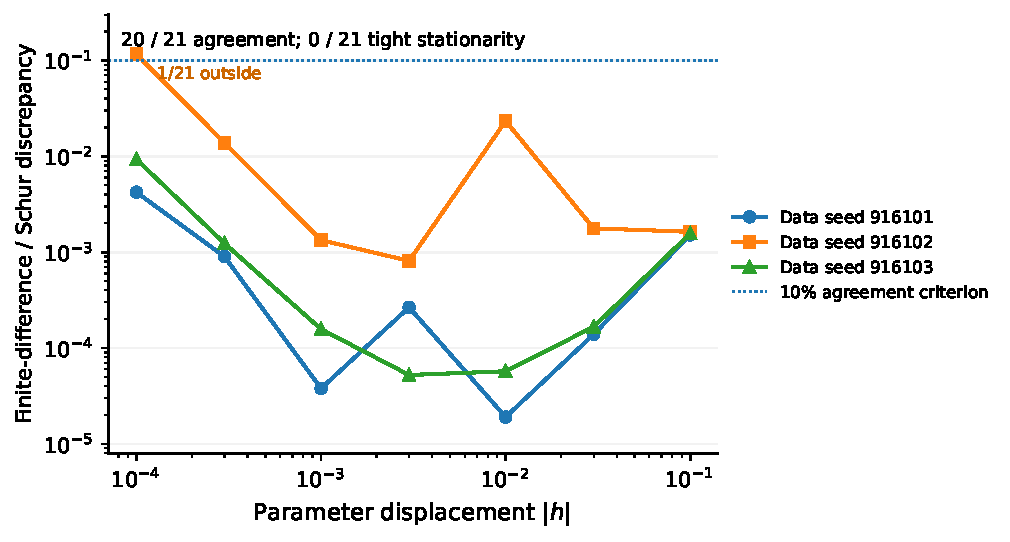
\includegraphics[width=.95\linewidth]{figures/fig06_profile_resolution.pdf}
\caption{Relative discrepancy $|D_\gamma(h;1)-\Hred|/\max(|\Hred|,10^{-8})$ across seven step sizes for three saturation data seeds.
Intermediate steps agree with $\Hred$ within the $10\%$ dotted threshold ($20/21$ points), whereas smaller steps amplify residual state-optimization error via $h^{-2}$ and $0/21$ branch pairs reach the strictest gradient tolerance.}
\label{fig:profile}
\end{figure}

\section{Discussion}
\label{sec:discussion}

\subsection{Implications for inverse-PINN diagnostics and interpreting \texorpdfstring{$\gamma$}{gamma}}
\label{sec:interpretation}

Routine post-training sensitivity checks in inverse PINNs freeze the trained network weights, suppressing a state-adaptation mechanism that operated throughout training.
Our results show that at weak damping ($\alpha=10^{-8}$) this omission is not a minor perturbation: across Burgers, Allen--Cahn, non-affine saturation, and coupled reaction--diffusion benchmarks, frozen-state curvature overestimates the $\gamma$-matched state-relaxed reference by roughly one to two orders of magnitude, whereas state elimination cuts relative error by one to four orders of magnitude.
Although the underlying Schur complement is classical, quantifying this bias, isolating its error budget, and supplying an energy-based solve-error bound make local state elimination directly applicable at well-converged inverse-PINN checkpoints.

Practitioners should interpret SAEPS not as a single parameter-free scalar, but as a local diagnostic indexed by the declared residual weights $W$, parameter coordinates, state metric, and damping $\gamma$.
Because $\gamma$ prices local weight motion, increasing $\gamma$ continuously suppresses state relaxation toward $\Fraw$; stronger damping reduces iterative solver cost and Gauss--Newton truncation simultaneously, but it changes the target $\Hred$ rather than merely stabilizing a fixed problem.
Any reported curvature or retained ratio $\eta$ should therefore state the residual metric and damping scale $\alpha$ explicitly.
Computationally, dense Cholesky reduction remains fastest for compact networks ($n_\theta\lesssim 10^2$--$10^3$), whereas matrix-free CG with the Proposition~2 energy audit provides a practical path when Jacobian storage becomes prohibitive.

\subsection{Limitations and scope boundaries}
\label{sec:limitations}

Four boundaries delimit the claims of this study and indicate where caution is required:
\begin{enumerate}
\item \textbf{Problem scale and dimensionality:} Trained accuracy benchmarks are restricted to one-dimensional synthetic PDEs with $n_\theta\in[33,337]$ state parameters. The $100{,}001$-parameter study employs a function-preserving expansion at $\alpha=10^{-2}$ and tests matrix-free operator feasibility rather than trained large-network accuracy. At weak damping ($\alpha=10^{-8}$), unpreconditioned CG iteration counts grow rapidly with ill-conditioning; scaling weak-damping solves to two- or three-dimensional trained PINNs will likely require spectral or low-rank Nystr\"om preconditioning.
\item \textbf{Center-convergence availability:} Exact-reference validation requires a valid state-stationary center with $H_{\theta\theta}+\gamma I\succ 0$. Three Burgers checkpoints, one Allen--Cahn checkpoint, two coupled checkpoints ($8/10$, below the prespecified $9/10$ gate), and all five wide Burgers stress runs failed state-center validity; invalid centers are retained in planned denominators and excluded from conditional error summaries.
\item \textbf{Finite-step nonlinear profile equivalence:} Although $20/21$ saturation finite differences fall within $10\%$ of $\Hred$, $0/21$ branch pairs reached the strictest gradient tolerance across scales. SAEPS is therefore validated against local exact-Hessian Schur references, not as a substitute for globally converged nonlinear likelihood profiles.
\item \textbf{Statistical inference and identifiability:} Block residual weights $W$ define an optimization metric rather than inverse observation-noise variances. Moreover, because $A_\gamma\succ 0$ for any $\gamma>0$, $\ker(\Fse)=\ker(\Jl^\top A_\gamma\Jl)=\ker(\Jl)$: positive damping preserves any nullspace already present in $\Jl$, prevents state-compensable directions outside $\ker(\Jl)$ from collapsing to exact zero, and yields $\Fse\succ 0$ whenever $\Jl$ has full column rank. Consequently, SAEPS does not by itself deliver calibrated frequentist confidence intervals, posterior covariances, or global structural identifiability guarantees, nor does it modify the fitted physical parameter $\lambda_0$.
\end{enumerate}

\section{Conclusions}
\label{sec:conclusions}

We quantified the curvature inflation introduced by freezing neural network weights during post-training inverse-PINN sensitivity analysis and corrected it via regularized state elimination (SAEPS).
At the prespecified damping $\alpha=10^{-8}$, SAEPS removes the dominant state-freezing bias across Burgers, Allen--Cahn, a non-affine saturation PDE, and trained networks spanning $65$--$337$ state parameters, recovering the exact relaxation correction to within $0.4\%$ median error and cutting curvature error relative to matched exact finite-$\gamma$ Schur references by one to four orders of magnitude.
An exact error decomposition, a sufficient dominance condition ($\chi<1$) satisfied on all $39/39$ valid scalar checkpoints, undamped-limit ill-conditioning audits, and an exact-arithmetic a posteriori energy bound provide a transparent framework for auditing local curvature and matrix-free solves.
Future work should address preconditioned matrix-free solvers for weak damping in two- and three-dimensional trained PINNs, principled damping selection tied to observation-noise scaling, and coupling state-relaxed curvature with bias-aware frequentist interval calibration.

\section*{Acknowledgments}
This work was supported by the National Key R\&D Program of China (Grant No. 2023YFB3307700), the China Postdoctoral Science Foundation (Grant No. GZC20252728, 2026M794817), and Jiangsu Province Outstanding Postdoctoral Fellowship Program (Grant No. 2025ZB735).

\section*{CRediT authorship contribution statement}
\noindent\textbf{Ziwei Ren:} Conceptualization; Methodology; Software; Validation; Formal analysis; Investigation; Data curation; Writing -- original draft; Writing -- review \& editing; Visualization.\\
\textbf{Shijin Zhang:} Resources; Supervision; Project administration; Funding acquisition.\\
\textbf{Ming Chen:} Conceptualization; Methodology; Data curation; Supervision; Writing -- review \& editing.\\
\textbf{Chuangrui Zheng:} Methodology; Validation; Supervision; Project administration.

\section*{Declaration of competing interest}
The authors declare that they have no known competing financial interests or personal relationships that could have appeared to influence the work reported in this paper.

\section*{Declaration of generative AI and AI-assisted technologies in the writing process}
During the preparation of this work, the authors used AI-assisted tools to assist with editorial drafting, language polishing, and manuscript consistency checks.
After using these tools, the authors reviewed, verified, and edited all content as needed and take full responsibility for the content of the published article.

\section*{Supplementary material}
Supplementary data, detailed cohort tables, damping sweeps, matched-damping timing ledgers, and additional figures are provided in the accompanying file \texttt{supplement.pdf}.

\section*{Data and code availability}
Source code, processed benchmark tables, figure- and table-generation scripts, algebraic verification tests, and archived experimental logs are available at \url{https://github.com/milumilelu/SAEPS}.
As documented in the Supplementary Material, all processed curvature blocks and saturation/architecture records are archived for reproduction, whereas original unarchived state tensors from the earlier scalar training runs are unavailable for independent tensor-level replay.

\begin{thebibliography}{99}

\small
\setstretch{1.0}
\setlength{\bibsep}{3.5pt}
\raggedright

\bibitem{raissi2019physics}
M.~Raissi, P.~Perdikaris, G.E.~Karniadakis,
Physics-informed neural networks: A deep learning framework for solving forward and inverse problems involving nonlinear partial differential equations,
\textit{J. Comput. Phys.} \textbf{378} (2019) 686--707.
\doi{10.1016/j.jcp.2018.10.045}.

\bibitem{karniadakis2021piml}
G.E.~Karniadakis, I.G.~Kevrekidis, L.~Lu, P.~Perdikaris, S.~Wang, L.~Yang,
Physics-informed machine learning,
\textit{Nat. Rev. Phys.} \textbf{3} (2021) 422--440.
\doi{10.1038/s42254-021-00314-5}.

\bibitem{hinze2009optimization}
M.~Hinze, R.~Pinnau, M.~Ulbrich, S.~Ulbrich,
\textit{Optimization with PDE Constraints},
Springer, Dordrecht, 2009.
\doi{10.1007/978-1-4020-8839-1}.

\bibitem{biros2005parallel}
G.~Biros, O.~Ghattas,
Parallel Lagrange--Newton--Krylov--Schur methods for PDE-constrained optimization. Part I: The Krylov--Schur solver,
\textit{SIAM J. Sci. Comput.} \textbf{27} (2005) 687--713.
\doi{10.1137/S106482750241565X}.

\bibitem{buithanh2013computational}
T.~Bui-Thanh, O.~Ghattas, J.~Martin, G.~Stadler,
A computational framework for infinite-dimensional Bayesian inverse problems. Part I: The linearized case, with application to global seismic inversion,
\textit{SIAM J. Sci. Comput.} \textbf{35} (2013) A2494--A2523.
\doi{10.1137/12089586X}.

\bibitem{haghighat2021physics}
E.~Haghighat, M.~Raissi, A.~Moure, H.~Gomez, R.~Juanes,
A physics-informed deep learning framework for inversion and surrogate modeling in solid mechanics,
\textit{Comput. Methods Appl. Mech. Engrg.} \textbf{379} (2021) 113741.
\doi{10.1016/j.cma.2021.113741}.

\bibitem{mishra2022inverse}
S.~Mishra, R.~Molinaro,
Estimates on the generalization error of physics-informed neural networks for approximating a class of inverse problems for PDEs,
\textit{IMA J. Numer. Anal.} \textbf{42} (2022) 981--1022.
\doi{10.1093/imanum/drab032}.

\bibitem{kharazmi2021identifiability}
E.~Kharazmi, M.~Cai, X.~Zheng, Z.~Zhang, G.~Lin, G.E.~Karniadakis,
Identifiability and predictability of integer- and fractional-order epidemiological models using physics-informed neural networks,
\textit{Nat. Comput. Sci.} \textbf{1} (2021) 744--753.
\doi{10.1038/s43588-021-00158-0}.

\bibitem{radfar2026sparse}
S.~Radfar,
How sparse and how noisy? Systematic benchmarking of inverse physics-informed neural networks for Manning friction estimation in shallow water equations,
\textit{Phys. Fluids} \textbf{38} (2026) 086611.
\doi{10.1063/5.0349054}.

\bibitem{zhang2026beyond}
Y.~Zhang, Q.~Tao,
Beyond field accuracy: Two-axis diagnosis of inverse-PINN parameter error,
arXiv preprint \href{https://arxiv.org/abs/2608.15373}{arXiv:2608.15373} (2026).
\doi{10.48550/arXiv.2608.15373}.

\bibitem{krishnapriyan2021characterizing}
A.S.~Krishnapriyan, A.~Gholami, S.~Zhe, R.M.~Kirby, M.W.~Mahoney,
Characterizing possible failure modes in physics-informed neural networks,
\textit{Adv. Neural Inf. Process. Syst.} \textbf{34} (2021) 26548--26560.

\bibitem{wang2022ntk}
S.~Wang, X.~Yu, P.~Perdikaris,
When and why PINNs fail to train: A neural tangent kernel perspective,
\textit{J. Comput. Phys.} \textbf{449} (2022) 110768.
\doi{10.1016/j.jcp.2021.110768}.

\bibitem{rathore2024loss}
P.~Rathore, W.~Lei, Z.~Frangella, L.~Lu, M.~Udell,
Challenges in training PINNs: A loss landscape perspective,
\textit{Proc. Mach. Learn. Res.} \textbf{235} (2024) 42159--42191.

\bibitem{muller2023engd}
J.~M\"uller, M.~Zeinhofer,
Achieving high accuracy with PINNs via energy natural gradient descent,
\textit{Proc. Mach. Learn. Res.} \textbf{202} (2023) 25471--25485.

\bibitem{yang2021bpinns}
L.~Yang, X.~Meng, G.E.~Karniadakis,
B-PINNs: Bayesian physics-informed neural networks for forward and inverse PDE problems with noisy data,
\textit{J. Comput. Phys.} \textbf{425} (2021) 109913.
\doi{10.1016/j.jcp.2020.109913}.

\bibitem{pensoneault2024eki}
A.~Pensoneault, X.~Zhu,
Efficient Bayesian physics informed neural networks for inverse problems via ensemble Kalman inversion,
\textit{J. Comput. Phys.} \textbf{508} (2024) 113006.
\doi{10.1016/j.jcp.2024.113006}.

\bibitem{hemachandra2025pied}
A.~Hemachandra, G.K.R.~Lau, S.-K.~Ng, B.K.H.~Low,
PIED: Physics-informed experimental design for inverse problems,
in: \textit{The Thirteenth International Conference on Learning Representations (ICLR)}, 2025.

\bibitem{golub1973variable}
G.H.~Golub, V.~Pereyra,
The differentiation of pseudo-inverses and nonlinear least squares problems whose variables separate,
\textit{SIAM J. Numer. Anal.} \textbf{10} (1973) 413--432.
\doi{10.1137/0710036}.

\bibitem{golub2003separable}
G.H.~Golub, V.~Pereyra,
Separable nonlinear least squares: The variable projection method and its applications,
\textit{Inverse Problems} \textbf{19} (2003) R1--R26.
\doi{10.1088/0266-5611/19/2/201}.

\bibitem{newman2021varpro}
E.~Newman, L.~Ruthotto, J.~Hart, B.~van Bloemen Waanders,
Train like a (Var)Pro: Efficient training of neural networks with variable projection,
\textit{SIAM J. Math. Data Sci.} \textbf{3} (2021) 1041--1066.
\doi{10.1137/20M1359511}.

\bibitem{dong2023inverse}
S.~Dong, Y.~Wang,
A method for computing inverse parametric PDE problems with random-weight neural networks,
\textit{J. Comput. Phys.} \textbf{489} (2023) 112263.
\doi{10.1016/j.jcp.2023.112263}.

\bibitem{uriarte2025least}
C.~Uriarte, M.~Bastidas, D.~Pardo, J.M.~Taylor, S.~Rojas,
Optimizing Variational Physics-Informed Neural Networks Using Least Squares,
\textit{Comput. Math. Appl.} \textbf{185} (2025) 76--93.
\doi{10.1016/j.camwa.2025.02.022}.

\bibitem{zhang2026bilo}
R.Z.~Zhang, C.E.~Miles, X.~Xie, J.S.~Lowengrub,
BiLO: Bilevel local operator learning for PDE inverse problems,
\textit{J. Comput. Phys.} \textbf{551} (2026) 114679.
\doi{10.1016/j.jcp.2026.114679}.

\bibitem{raue2009structural}
A.~Raue, C.~Kreutz, T.~Maiwald, J.~Bachmann, M.~Schilling, U.~Klingm{\"u}ller, J.~Timmer,
Structural and practical identifiability analysis of partially observed dynamical models by exploiting the profile likelihood,
\textit{Bioinformatics} \textbf{25} (2009) 1923--1929.
\doi{10.1093/bioinformatics/btp358}.

\end{thebibliography}
\end{document}
